\documentclass{article}

\usepackage{graphicx}

\title{Prilimary Algorithm for Horn Classification.}

\begin{document}
\maketitle

\section{Priliminary Classification}

We record audio 1 second chunks of audio data and pass it through a CNN classifier network. A pretrained classifier trained on youtube data known as YAMNet is
used for this perpose. This classifies the data into 512 different chunks, and returns an encoding vector,which is later used for further classifying horndata.

The YAMNet network has the following classes which are relevant for us:

\begin{itemize}
    \item Vehicle
    \item Vehicle Horn
    \item Car Horn
    \item Air Horn, Truck Horn
    \item Bicycle Bell
    \item Honk
\end{itemize}

The model is simple enough that we maybe able to transmit this data over the wire to a centralized server for further processing.

\section{Principle Component Analysis and Clustering}

To further improve the classification granularity we add a PCA layer which effectively reduces the irrelevant dimentions from the 1024 dimentional data. We also 
perform extractions on label by first sorting the probabilty vector in descending order and picking the first `n' elements whose sum is greater than 95\%.

After this processing we pass the PCA embeddings to an real-time classifier calle Birch. This clusters together all the different kinds of horns into different section.
We can ensure we only classify horns by limiting our search to the previously mentioned classes.

\section{Labeling Data by using LLMs}

To label the clusters created by Birch we utilize an LLM such as ollama. We pass the labels that have been collected through the duration of data collection. This allowsj
the LLMs to predict which class the audio could belong to. Effectively giving us the vehicle where the horn originated. The classes Car/Truck are present, motorbike is not however a Motorcycle noise is a classifier catagory in YAM thus the LLM may be able to extract this information out of the system.

We are running the ollama LLM locally on the machine to avoid having to connect to a resource expensive network connection.

\section{Problems present in current method}
There are a few issues in the current method.

\begin{itemize}
    \item The Audio data is highly dependent on the recording system and the environment.
    \item The LLMs (locally run) tend to hallucinate data, thus sometimes misnaming some catagories.
    \item Unstructured output from LLMS
    \item The Clustering has to happen at higher than 5dims to be effective.
\end{itemize}

However dispite these issues, The YAM network provides us with enough flexibility that we may be able to proceed.

\section{Graphs after training.}

This is an example of this algorithm at work. I have not enabled the filtering of different audio to check if the LLM worked correctly, and unfortunately due to the small parameter count it hallucinated a lot.

\begin{figure}
    \centering
    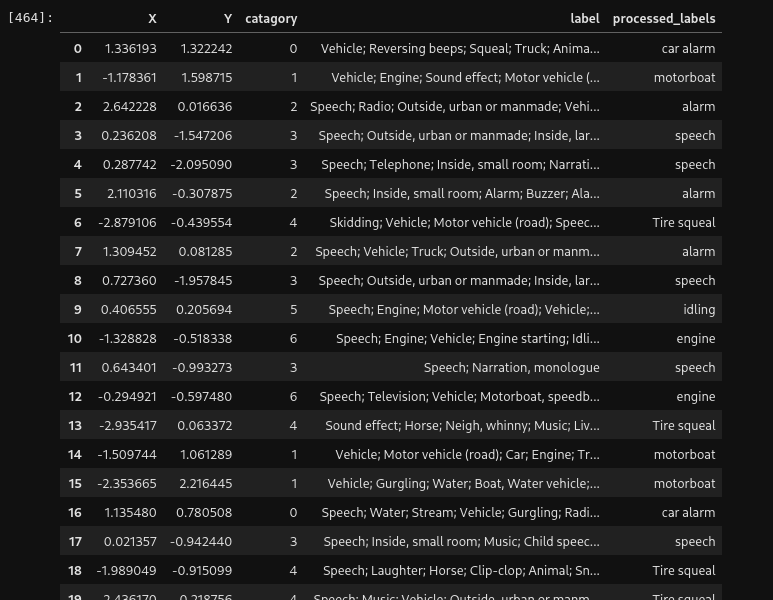
\includegraphics[width=\textwidth]{Screenshot From 2026-05-14 19-42-21-1.png}
    \caption{Example of classifcation of generated vector.}
\end{figure}
\begin{figure}
    \centering
    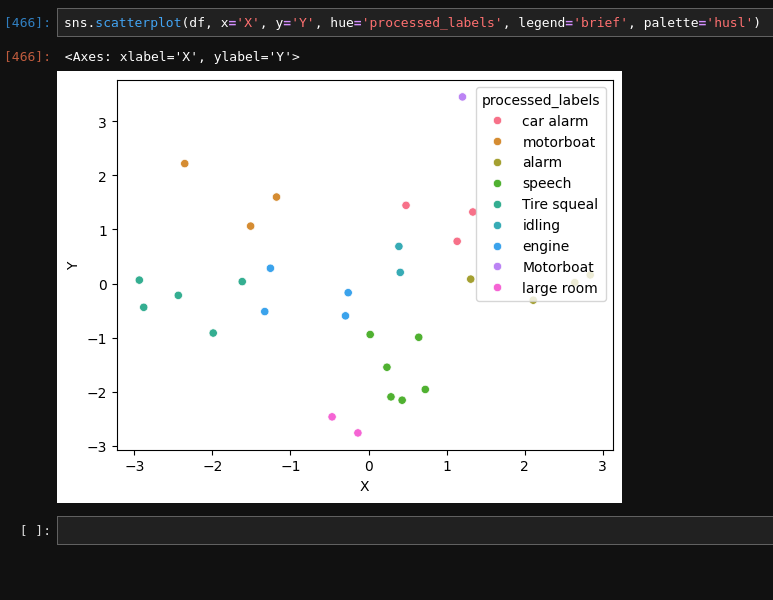
\includegraphics[width=\textwidth]{Screenshot From 2026-05-14 19-42-40.png}
    \caption{After Clustring graph.}
\end{figure}

\end{document}
